\documentclass[exercice,a4]{thedocument}%
\usepackage{texmaths-tikz}%
\usepackage{enumitem}%
\usepackage[np]{numprint}%
\startdatakeys
\source{24GENMATG11}
\BO{2026}
\cycle{4}
\competencesDuSocle{CA,RA}
\objectifsApprentissage{C4A1aa,C4A1aj,C4A2ad,C4A2bb,C4A2ac}
\motsCles{circuits,durée,facteurs premiers,multiple,PGCD,PPCM}
\enddatakeys
\begin{document}%
Un entraîneur prépare deux circuits d'entraînement :
\begin{itemize}[label=\textbullet]
    \item un circuit commence à l'exercice 1 et se termine en revenant à
    l'exercice 1 ;
    \item le circuit 1 contient cinq exercices de 40 secondes, suivis chacun
    de 16 secondes de repos ;
    \item le circuit 2 contient dix exercices de 30 secondes, suivis chacun
    de 5 secondes de repos.
\end{itemize}

\begin{center}
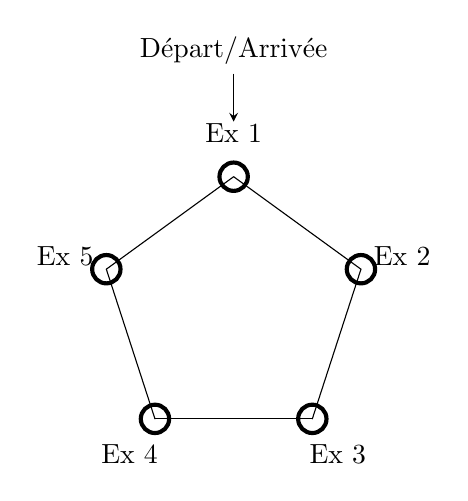
\begin{tikzpicture}[line cap=round]
    \draw[<-,>=stealth](0,2.4)--(0,3)node[above]{Départ/Arrivée};
    \foreach \ex in {1,...,5}{
        \draw[line width=1.5pt](162-\ex*72:1.7)circle(.18);
        \node at(162-\ex*72:2.25){Ex~\ex};
        \draw(162-\ex*72:1.7)--(90-\ex*72:1.7);
    }
\end{tikzpicture}
\hspace{20pt}
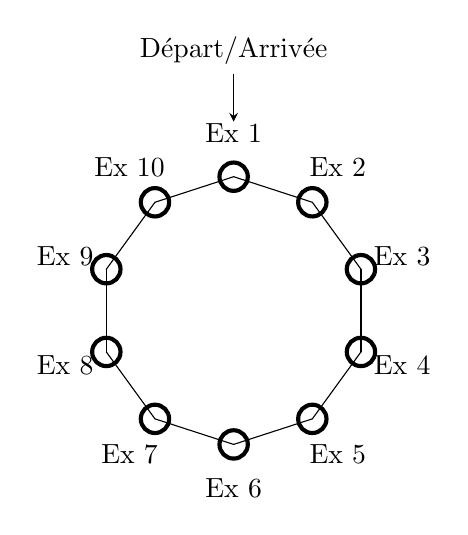
\begin{tikzpicture}[line cap=round]
    \draw[<-,>=stealth](0,2.4)--(0,3)node[above]{Départ/Arrivée};
    \foreach \ex in {1,...,10}{
        \draw[line width=1.5pt](126-\ex*36:1.7)circle(.18);
        \node at(126-\ex*36:2.25){Ex~\ex};
        \draw(126-\ex*36:1.7)--(90-\ex*36:1.7);
    }
\end{tikzpicture}
\end{center}

\begin{enumerate}
    \item Montrer que le circuit 1 s'effectue en 280 secondes et que le
    circuit 2 s'effectue en 350 secondes.
    \item Donner la décomposition en produit de facteurs premiers de 280 et
    de 350.
    \item Une séance est constituée de plusieurs tours du même circuit.
    \begin{enumerate}
        \item Expliquer pourquoi, après $\np[s]{2800}$, Camille se trouve de
        nouveau au départ du circuit 1. Préciser où se trouve Dominique.
        \item Après le coup de sifflet, combien de temps faut-il pour que
        Camille et Dominique se retrouvent pour la première fois au départ de
        leur circuit ? Exprimer cette durée en minutes et secondes.
    \end{enumerate}
\end{enumerate}
\showthesource
\end{document}
